\chapter{Kinematic Model of Non-holonomic omnidirectional mobile robot}
\label{cha:Kinematic}

Kinematics is the most basic study of how mechanical systems behave. In our case, Kinematics make a connection between joint states(driving rate, steering angle and steering velocity) and platform velocity in the 
task space. Which is fundmental for our control method.
First, a overview of the mobile platform is given (\cref{sec:model_overview}).
Afterwards, the Forward and Inverse Kinematic equations (\cref{sec:hum}) are presented.
%\cref{sec:application} explains how the model is implemented in different model predictive control (MPC) approaches.

\section{Model overview}
\label{sec:model_overview}

The the platform is a regid squre body with four conventional wheels on each corner. each wheel can be controlled independently (steering/driving).

In the task space, the frame is as shown in \cref{fig:taskSpace} we use $ \xi = [x,t,\theta]$ to discribe the current platform position and orientation, use $ \dot{\xi} = [\dot{x},\dot{y},\dot{\theta}] $ and 
$ \ddot{\xi}= [\ddot{x},\ddot{y},\ddot{\theta}] $ to discribe the platform velocity and acceleration. 

In the following discussion, we will mainly focus on to frames, world frame in which the odometry $ \hat{\xi} $ is calculated, and body frame in which the platform velocity $\hat{\dot{\xi}}^b$ and platform 
acceleration $ \hat{\ddot{\xi}}^b $ is calculated, the command from global planer $ \dot{\xi}^b $ and $ \ddot{\xi}^b $ is also assumed to be in the body frame. The lower case "b" in the upper corner indicates 
this variable is expressed in the body frame. While the notion with "hat" like $\hat{}$  is used to expressed the measured feedback.

\begin{figure}[t]
	\begin{center}
	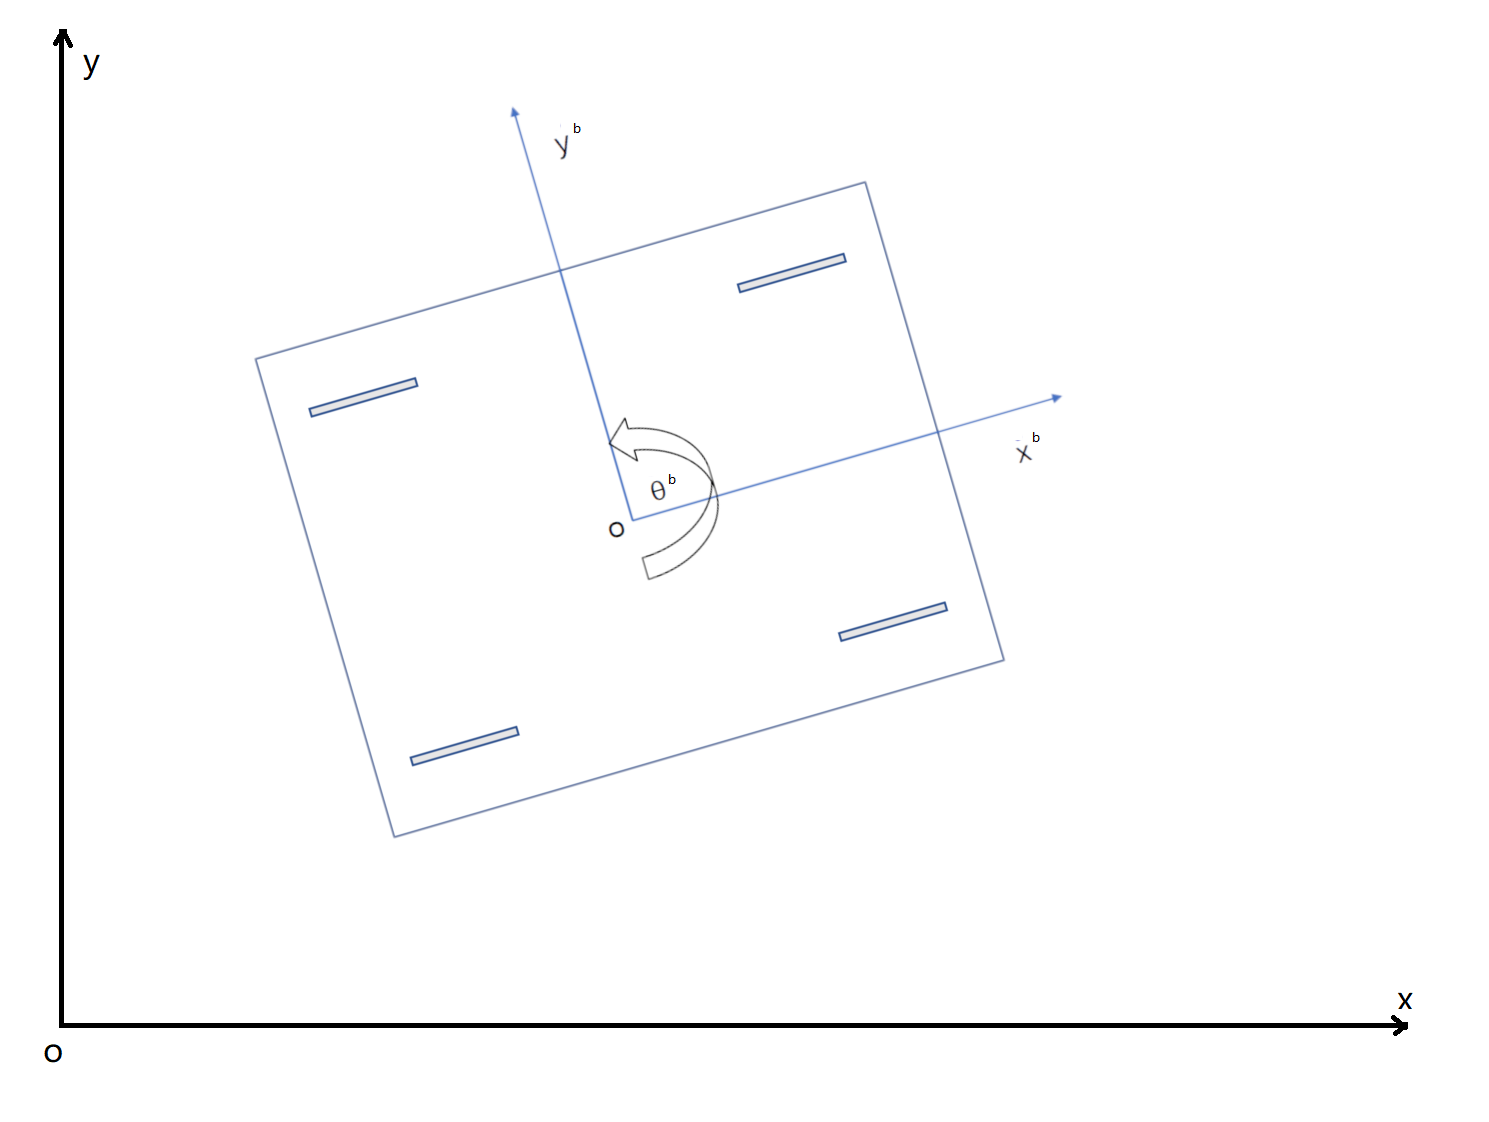
\includegraphics[width=\textwidth]{../Figures/frame.png}
	\caption{Task space}
	\label{fig:taskSpace}
	\end{center}
\end{figure}


In the joint space we use $\beta_{i}$ and $\dot{\beta_{i}}$ to discribe the steering angle and steering velocity of the wheel, and $\dot{\phi}$ for driving velocity, which is shown in figure \cref{fig:wheel}. The measured
feedback from sensor is noted with $\hat{}$ while the joint space commands are with out special notion.

\begin{figure}[t]
\begin{center}
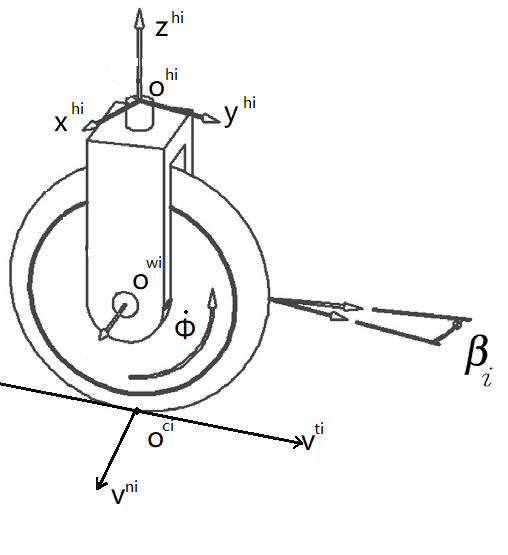
\includegraphics[width=.7\textwidth]{../Figures/wheel.png}
\caption{Wheel structure}
\label{fig:wheel}
\end{center}
\end{figure}

\begin{equation}\label{eq:venflux}
V_{ven,flux} = D_{ws} \cdot \alpha \cdot U_{ven}^\beta + c_{loss} \cdot D_{ws} + c_{leak},
\end{equation} 
where $\alpha$ and $\beta$ are empirical parameters, $c_{loss}$ is the influence factor of the windspeed when the vents are closed and $c_{leak}$ is the leakage of warmth due to imperfect sealing.
In the following two sections the two ODEs are explained.
The value of the parameters are gathered in \cref{sec:physical_params}.
%%%%%%%%%%%%%%%%%%%%%%%%%%%%%%%%%%%%%%%%%%%%%%%%%%%%%%%%%%%%%%%%%%%%%%%%%%%%%
\section{Internal air temperature model}
\label{sec:temp}
The greenhouse air temperature is modelled by the following balance:
\begin{equation}\label{eq:temp}
\begin{split}
\frac{dX_{T,a}}{dt} &= \frac{c_{area,ss} \cdot c_{sph,a} \cdot c_{den,a}}{c_{vol,g}} \cdot \left(Q_{sol,a} + Q_{cnv,ss-a} + Q_{heat-a} \right.\\
		& \left. + Q_{cnv-cnd,a-e} - Q_{ven,a-e} - Q_{loss,a-e} - Q_{trp,cr}\right),
\end{split}
\end{equation}
where $c_{area,ss}$ is the surface area of the soil, $c_{sph,a}$ is the specific heat and $c_{den,a}$ is the density of the air.
The heat fluxes $Q_{(\cdot)}$ are described in the following paragraphs.

The solar radiation absorbed by the air $Q_{sol,a}$ is given by:
\begin{equation}\label{eq:rs}
Q_{sol,a} = c_{asw,a} \cdot V_{tsw,g} \cdot D_{rs,e} \cdot \left( 1 - U_{shd} \right),
\end{equation}
where $c_{asw,a}$ is the short-wave absorption coefficient of the greenhouse air. $V_{tsw,g}$ is the short wave heat transmission coefficient depending on the cover, its whitening state and the shading screen.

The heat transfer between the soil surface and the inside air is depending on the temperature difference between soil surface temperature $D_{T,ss}$ and inside air temperature $X_{T,a}$:
\begin{equation}\label{eq:ss}
Q_{cnv,ss-a} = c_{cnv,ss-a} \cdot (D_{T,ss}-X_{T,a}),
\end{equation}
where $c_{cnv,ss-a}$ is the constant convection coefficient.

This process is proportional to the temperature difference between outside air temperature $D_{T,e}$ and inside air temperature $X_{T,a}$:
\begin{equation}\label{eq:a-e}
Q_{cnd-cnv,a-e} = c_{cnd-cnv,a-e} \cdot (D_{T,ss}-X_{T,a}),
\end{equation}
where $c_{cnd-cnv,ss-a}$ is the thermal loss coefficient for convection and conduction processes.

The Heat transfer to the outside air due to ventilation and infiltration are described by:
\begin{equation}\label{eq:loss}
\begin{split}
Q_{ven,a-e} + Q_{loss,a-e}& = \\
\frac{c_{den,a} \cdot c_{sph,a}}{c_{area,ss}} \cdot &V_{ven,flux} \cdot (X_{T,a}-D_{T,e}).
\end{split}
\end{equation}
%%%%%%%%%%%%%%%%%%%%%%%%%%%%%%%%%%%%%%%%%%%%%%%%%%%%%%%%%%%%%%%%%%%%%%%%%%%%%%%%%%%%%%%%%%%%%%%%%%%%%%%%%%%%%%%%%%%%%%%%%%%%%%%%%%%%%%%%%%%%%%%%%%%%%%%%%%
%%%%%%%%%%%%%%%%%%%%%%%%%%%%%%%%%%%%%%%%%%%%%%%%%%%%%%%%%%%%%%%%%%%%%%%%%%%%%%%%%%%%%%%%%%%%%%%%%%%%%%%%%%%%%%%%%%%%%%%%%%%%%%%%%%%%%%%%%%%%%%%%%%%%%%%%%%

\section{Internal air humidity model}
\label{sec:hum}
The internal air humidity is modelled by the following balance:
\begin{equation}\label{eq:hum}
\frac{dX_{H_{a,a}}}{dt} = \frac{c_{area,ss}}{c_{den,a} \cdot c_{vol,g}} \cdot \left(M_{trp,cr}-M_{ven,a-e}+U_{hum}\right),
\end{equation}
where the two sources of water vapor are the crop transpiration $M_{trp,cr}$ and the injections of the moisturisation system $U_{hum}$, while the loss of water vapor is due to exchange of air with the outside through ventilation.

For the water vapour increase due to the crop tomato a balance $M_{trp,cr}$ based on the Penman-Monteith equation is used:
\begin{equation}\label{eq:crtp}
\begin{split}
M_{trp,cr} &= \frac{1}{V_{r,trp}}\Big(V_{hsat,a} \\
           &+ \frac{1}{c_{den,a}}\frac{V_{ssvp}}{c_{psyco}}\frac{V_{r,bl}}{2D_{LAI}}\frac{V_{rn,cr}}{V_{lt,vap}}-X_{Ha,a} \Big),
\end{split}
\end{equation}
where $c_{psyco}$ is the thermodynamic psychometric constant, $D_{LAI}$ is the leaf area index of the tomato crop and $c_{den,a}$ is the densitiy of the inside air.

The thermodynamic psychometric constant $c_{psyco}$ is calculated by:
\begin{equation}\label{eq:psyco}
c_{psyco} = \frac{c_p \cdot p}{\lambda_v \cdot MW_{ratio}},
\end{equation}
where $p$ is the atmospheric pressure, $\lambda_v$ is the latent heat of water vaporization, $c_p$ is the specific heat of air at constant pressure and $MW_{ratio}$ is the ratio of molecular weight of water vapour and dry air.

The water concentration of the air at saturation $V_{hsat,a}$ is calculated with Teten's formula:
\begin{equation}\label{eq:vhsat}
V_{hsat,a} = 611.2 \cdot exp\left({\frac{\frac{17.62 \cdot X_{T_{a,a}}}{243.12 + D_{T,e}}}{R_D \left(273.2 + X_{T_{a,a}}\right)}}\right),
\end{equation} where $R_D$ is the gas constant of water vapor.

The transpiration resistance $V_{r,trp}$ is described by:
\begin{equation}\label{eq:vrtrp}
V_{r,trp} = \frac{1}{2D_{LAI}}\left[\left(1+\frac{V_{ssvp}}{c_{psyco}}\right)V_{r,bl}+V_{r,s}\right],
\end{equation}
where $V_{r,bl}$ is the boundary layer resistance \cref{eq:vrbl} and $V_{r,s}$ is the stomatal resistance \cref{eq:vrs}.

\begin{equation}\label{eq:vrbl}
V_{r,bl} = 220 \cdot \frac{c_{cl,cr}^{0.2}}{V_{ws,a}^{0.8}}
\end{equation}
where $c_{cl,cr}$ is the characteristic length of the crop leaf and and $V_{ws,a}$ is the average inside air speed:
\begin{equation}\label{eq:airspeed}
V_{ws,a} = \frac{V_{ven,flux}}{c_{area,p}},
\end{equation}
where $c_{area,p}$ is the the cross section area the air is streaming through. 

The slope of the saturated vapor pressure curve $V_{ssvp}$ is calculated by this empirical balance:
\begin{equation}\label{eq:ssvp}
V_{ssvp} = 0.04145 \cdot e^{0.060888 \cdot X_{T,a}}.
\end{equation}

Because the stomatal resistance of the tomato crop is mainly affected by global radiation, it can be described by:
\begin{equation}\label{eq:vrs}
V_{r,s}=200\left(1+\frac{1}{e^{0.05 \cdot V_{tsw,g} \cdot D_{rs,e} - 50}}\right),
\end{equation}
where $V_{tsw,g}$ is the short wave heat transmission coefficient depending on the cover, its whitening state and the shading screen.

$V_{lt,vap}$ is the latent heat of evaporation of water calculated at internal air temperature using:
\begin{equation}\label{eq:vltvap}
V_{lt,vap} = 4185.5 \cdot \left(597.0 - 0.56 \cdot X_{T,a}\right).
\end{equation}

The loss of water vapour due to natural ventilation and infiltration $M_{ven,a-e}$ is described by:
\begin{equation}\label{eq:mven}
\begin{split}
M_{ven,a-e} &= \frac{c_{den,a}}{c_{area,ss}} \cdot V_{ven,flux} \cdot \left(X_{H_{a,a}}-D_{H_a,e}\right) \\
            &+ M_{loss,a-e},
\end{split}
\end{equation}
where $M_{loss,a-e}$ are constant infiltration losses.\par\medskip

Establishing a (pseudo-) physical greenhouse model was illustrated in this chapter.
The model contains nonlinear ODEs for the inside air temperature and humidity. 
The nonlinear greenhouse model will be used as the prediction model for nonlinear MPC.
For linear MPC an analytical linearization will be derived.
In the following chapter the theoretical fundamentals of MPC are presented.